\documentclass{article}
\usepackage{fontenc}
\usepackage[ngerman]{babel}
\usepackage[utf8]{inputenc}
\usepackage{graphicx}
\usepackage{grffile}
\usepackage{subcaption}
\usepackage[export]{adjustbox}
\graphicspath{ {./pics} }
\DeclareUnicodeCharacter{2028}{\linebreak}
\usepackage{hyperref}
\usepackage{listings}
\usepackage{color}

\definecolor{dkgreen}{rgb}{0,0.6,0}
\definecolor{gray}{rgb}{0.5,0.5,0.5}
\definecolor{mauve}{rgb}{0.58,0,0.82}

\lstset{frame=tb,
  language=Java,
  aboveskip=3mm,
  belowskip=3mm,
  showstringspaces=false,
  columns=flexible,
  basicstyle={\small\ttfamily},
  numbers=left,
  numberstyle=\tiny\color{gray},
  keywordstyle=\color{blue},
  commentstyle=\color{dkgreen},
  stringstyle=\color{mauve},
  breaklines=true,
  breakatwhitespace=true,
  tabsize=3
}
\usepackage{datetime}
\newdateformat{myformat}{\THEDAY{ten }\monthname[\THEMONTH], \THEYEAR}

\begin{document}
	\begin{titlepage}
		\centering
		{\scshape\LARGE
			Ereignisdiskrete Systeme
			\par}
		\vspace{1.5cm}
		{\huge\bfseries Praktikum Blatt 1\par}
		\vspace{1.5cm}
		{\LARGE\itshape Jan Kristel, Alexandra Moritz\par}
		\vfill
			Aufsicht von Frau Rembold\par
			
		\vfill	
			{\large \today \par}	
		
	\end{titlepage}
	
	\tableofcontents
	\newpage
	\section{Aufgabe 1: MATLAB Grundlagen}
		\subsection{Was ist MATLAB?}
		Matlab ist eine Hochleistungssprache für technisches Rechnen. Es integriert Berechnung, Visualisierung und Programmierung in einer benutzerfreundlichen Umgebung, in der Probleme und Lösungen in vertrauter mathematischer Notation ausgedrückt werden. \\
		Typische Verwendungen sind:
		\begin{itemize}
			\item Mathematik und Rechnen
			\item Entwicklung von Algorithmen
			\item Modellierungssimulation und Visualisierung
			\item wissenschaftliche und technische Grafiken
		\end{itemize}
		Dies ermöglicht es Ihnen, viele, technische Rechenprobleme, insbesondere solche mit Matrix- und Vektorformulierungen, in einem Bruchteil der Zeit zu lösen, die benötigt würde, um ein Programm in einer skalaren, nicht-interaktiven Sprache wie C oder Fortan zu schreiben. Der Name Matlab steht für Matrixlabor.
		\subsection{Wesentliche Komponenten der MATLAB-Oberfläche}
			\begin{figure}[h]
				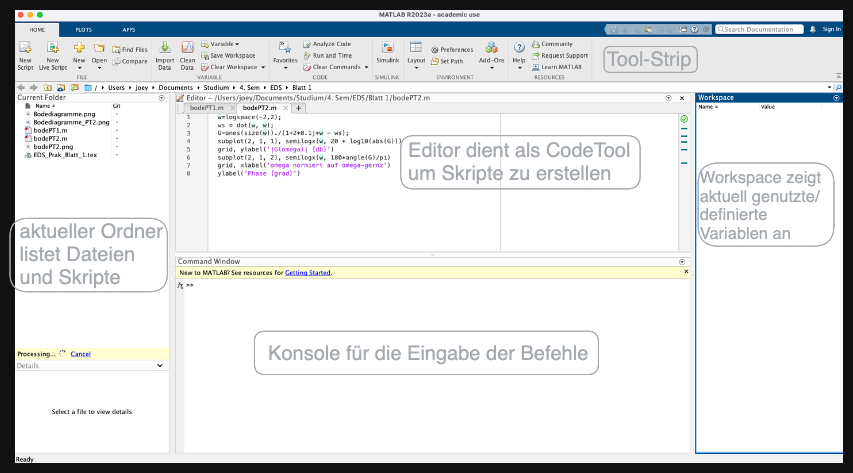
\includegraphics[scale=0.4]{./MATLAB_Oberflaeche_1_b.png}
				\caption{MATLAB Oberfläche}
				\label{fig1: MATLABOberflaeche}
			\end{figure}
	\newpage
			\begin{figure}
				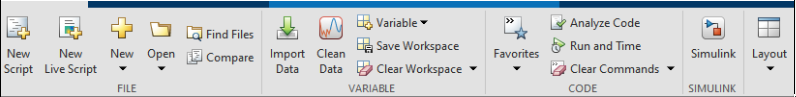
\includegraphics[scale=0.45]{./TOOLStirp.png}
				\caption{Tool-Strip im Reiter "Home". Hier lassen sich neue Skripte erstellen oder vorhandene öffnen.}
				\label{fig2: ToolStrip_Home}
			\end{figure}		

			\begin{figure}
				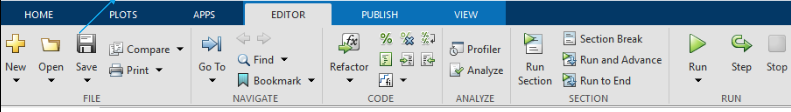
\includegraphics[scale=0.45]{./TOOLStrip_Editor.png}
				\caption{Tool-Strip im Reiter "Editor". Mit "Run" lassen sich die Programme/Skripte starten, die man im Editor erstellt hat.}
				\label{fig3: ToolStrip_Editor}
			\end{figure}	
		
		\subsection{\textit{Current Folder Browser} - Wozu? Was ist zu beachten?}
			Der Current Folder Browser zeigt Ordner und Dateien im aktuellen Arbeitsverzeichnis an. Man braucht es um den Zugriff auf die Dateien und Skripte zu erleichtern und um sicherzustellen das MATLAB die Dateien findet. Es ist wichtig die Dateien in der richtigen Stelle zu speichern, da die MATLAB-Programme standardgemäß im aktuellen Arbeitsverzeichnis ausgeführt werden. 
		
		\subsection{\textit{Comand Window} - Was verbirgt sich dahinter?}
			Das Command Window ist eine Konsole, die für die Eingabe von dem Benutzer verwendet wird und hier werden die MATLAB-Befehle eingegeben. Es wird auch eine Historie der davor eingegebenen Befehle gespeichert, sodass man sie immer wieder benutzen kann.
			
		\subsection{\textit{Tool-Strip} - Was verbirgt sich dahinter?}
			Der Tool-Strip ist eine Symbolleiste, hier findet man auf häufig verwendete Funktionen. Es bietet beispielsweise schnellen Zugriff auf das Command Window oder die Hilfe-Funktionen. 
		
		\subsection{Zweck des \textit{Workspaces}}
			Der Workspace zeigt die aktuellen Variablen und ihre Werte an. Man kann es vergleichen mit einer Variablenansicht in anderen Programmierumgebungen. Wird diser gelöscht bzw. \textit{gecleared}, sind alle benutzten Variablen nicht mehr definiert und nachfolgende Eingaben oder Scripte, die diese Variablen benutzten oder benutzt haben bringen einen Fehler.
		
		\subsection{Möglichkeiten Information von \textit{MATLAB-Hilfe} zu bekommen}
			\begin{itemize}
				\item Die Online-Hilfe von MATLAB, die über der Webseite erreichbar ist 
				\item in MATLAB direkt die Hilfefunktion, die über der Schaltfläche „Hilfe“ auf der Symbolleiste aufgerufen werden kann. Oder durch Eingabe in der Kommandozeile mit „help“. 
			\end{itemize}
		
		\subsection{Simulink}
			\begin{itemize}
				\item MATLAB öffnen
				\item in der Kommandozeile "simulink" eingeben
				\item oder über die Symbolleiste (Tool-Strip) Simulink starten
			\end{itemize}
		
		\subsection{\textit{Control System Tollbox} - Was ist das? Wo findet man sie?}
			Die \textit{Control System Toolbox} ist eine Add-On Bibliothek für MATLAB. Sie bietet Algorithmen und Apps zum systematischen Analysieren, Entwerfen und Optimieren linearer Steuerungssysteme. Sie können Ihr System als Übertragungsfunktion, Zustandsraum, Nullpolverstärkung oder Frequenzgangmodell spezifizieren. Beispielswiese mit dem Sprungantwortdiagramm und dem Bode-Diagramm lässt sich das Systemverhalten im Zeit- und Frequenzbereich analysieren und visualisieren. \\
			Die Toolbox stimmt automatisch sowohl SISO- als auch MIMO-Kompensatoren ab, einschließlich PID-Regler. Sie können verstärkungsgeplante Regler optimieren und mehrere Optimierungsziele festlegen. Man kann Designs validieren, indem man Anstiegszeit, Überschwingen, Einschwingzeit, Verstärkungs- und Phasenreserven und andere Anforderungen überprüfen. \\
			Zu finden ist die Erweiterung im \textit{AddOn-Explorer}. Diesen wird geöffnet in dem man im Reiter "Home" im Tool-Strip auf den Button \textit{AddOns} klickt.
		
		\subsection{Stateflow}
			\begin{itemize}
				\item MATLAB öffnen
				\item in der Kommandozeile "stateflow" eingeben und "Enter" drücken.
			\end{itemize}
		
		
	\newpage	
	\section{Aufgabe 2: Bodediagramme}
		\begin{figure}[h]
 		 	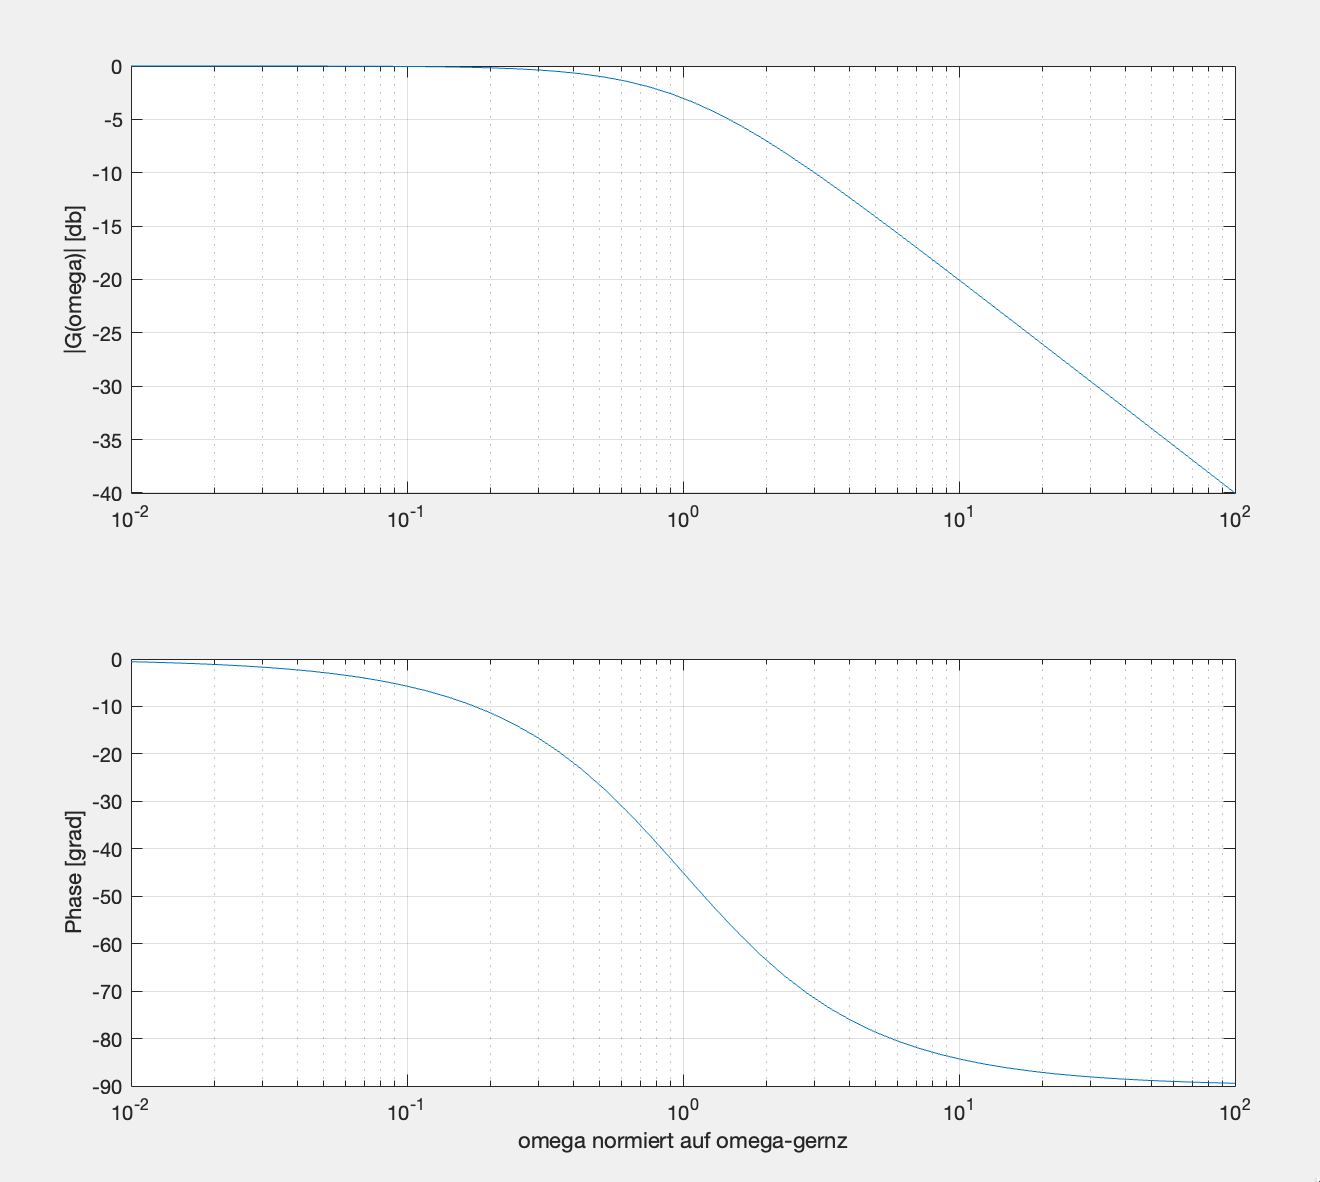
\includegraphics[scale=0.3, center]{./Bodediagramme.png}
			\caption{Bodediagramme entstanden aus bodePT1.m}
			\label{fig1: Bodediagramm1}
		\end{figure}
		\begin{lstlisting}
			w = logspace(-2,2);
			G = ones(size	(w))./(1+j*w);
			subplot(2, 1, 1), semilogx(w, 20 * log10(abs(G)))
			grid, ylabel('|G(w)| [db]')
			subplot(2, 1, 2), semilogx(w, 180*angle(G)/pi)
			grid, xlabel('w normiert auf w-gernz')
			ylabel('Phase [grad]')
		\end{lstlisting}
		Der oben gegebene Code erzeugt für ein PT1-Glied das zughörige Bodediagramm (Abb.4).
		% - erstellt Vector mit Werten zwischen 10^-2 und 10^2
		% - erstellt Vector G enthält 
			% - size(w) 1 kreuz N Matrix; N = # Elemente in w entspricht Array mit N
			% Elementen
			% - ones(size(w)) erstellt 1 kreuz N Matrix, an jedem Index mit 1 befüllt
			% - ./ teilt Elementweise jeden Wert des Arrays/Matrix durch das komplexe
			% Ergebnis des Nenners
			% - G ist der Ergebnis Array/die Matrix
			% - subplot erstellt ein Raster/Matrix mit (x, y, ) Achse. Der 3. Wert gibt
			% die Position des aktuellen Subplot an
			% - semilogx erstellt Plot mit logarithmische X-Achse, linearer y-Achse.
			% (x, y) gib die Daten für die entsprechende Achse
			% erstellt zweiten Plot mit den (x, y) Werten für (w, WInkel in Grad)
		\subsection{Normierter Frequenzgang PT1-Glied}
			Um die normierte Form der Übertragsfunktion zu bekommen, nimmt statt der Variablen \textbf{s} im laplace-transformiereten Bereich, die im komplexen und Frequenzbereich $j\omega$. 
			$$G(j\omega) = \frac{K_p}{\Big(1 + j\omega \cdot T\Big)}$$
\vspace{5mm}		
		\subsection{Normierter Frequenzgang PT2-Glied}
			$$G(j\omega) = \frac{K_p}{(j\omega)^2 + 2\cdot d\cdot \omega_0 \cdot j\omega + \omega_0^2}$$
\vspace{5mm}
		\subsection{Bodediagramm PT2-Glied}
			Für die Darstellung eines PT2-Glied wird der, unter Punkt 2 gezeigte Code wie folgt angepasst.
\vspace{5mm}
			\begin{lstlisting}
				Kp = 1;
				D = 0.1;

				w=logspace(-2,2);
				s= 1j .* w;
				G=ones(Kp)./(1 + 2*D*s - w.^2);
				subplot(2, 1, 1), semilogx(w, 20 * log10(abs(G)))
				grid, ylabel('|G(omega)| [db]')
				subplot(2, 1, 2), semilogx(w, 180*angle(G)/pi)
				grid, xlabel('omega normiert auf omega-gernz')
				ylabel('Phase [grad]')
			\end{lstlisting}
\vspace{5mm}
			Die Zeile, auf die es zu Achten gilt ist Zeile 6. Hier musste die Formel von einem PT1-Glied angepasst werden für ein PT2-Glied. \\
			Die Übertragsfunktion für ein PT2-Glied sieht folgender Maßen aus:
\vspace{5mm}			
			$$G(s) = \frac{Kp \cdot \omega_0^2}{s^2 + 2 \cdot D \cdot \omega_0^2 \cdot s + \omega_0^2}$$
\newpage
			Diese Formel wird für den Code angepasst. Die Resonanzfrequenz $\omega_0^2$ beginnt hier bei $1$. $s$ ist definiert aus durch $s = 1j \cdot \omega$. Da in der Formel $s^2$ verwendet wird verändert sich der Nenner der Übertragungsfunktion

			$$s^2 + 2 \cdot D \cdot s + 1$$

			$$= (j\omega)^2 + 2 \cdot D \cdot s + 1 $$

			$$= j^2 \cdot \omega^2 + 2 \cdot D \cdot s + 1 $$

			$$= - \omega^2 + 2 \cdot D \cdot s + 1$$

			$$= 1 + 2 \cdot D \cdot s - \omega^2 $$
			
			Diese Zeile in die Übertragungsfunktion eingesetzt, sieht dann wie folgt aus:
			
			$$G(s) = \frac{Kp}{1 + 2 \cdot D \cdot s - \omega^2}$$
			
			Diese Formel stimmt nun mit Zeile 6 aus dem Code überein und liefert das nachfolgende Bodediagramm.
			\begin{figure}
				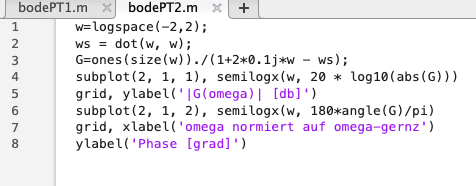
\includegraphics[scale = 0.3, center]{./bodePT2.png}
				\caption{Bodediagramm entstanden mit den Code aus 2.3}
				\label{fig2: Bodediagramm}
			\end{figure}
\newpage
	\section{Aufgabe 3: Ortskurve}
		Die Ortkurve ist eine graphische Darstellung des Frequenzgangs. Sie wird erstellt, indem man die den Frequenzbereich durchläuft, d.h. es werden einzelnen Werte (per Hand) oder alle Werte in die Übertragungsfunktion eingesetzt und etwaige Ergebnisse in den Koordinaten eingetragen.\\
		Für die Ortskurve wird nicht die laplace transformierte Übertragfunktion mit s verwendet, sondern die normiert $j\omega$.
	
		\subsection{Ortskurven}
			\subsubsection{a.1}
				$$G(s) = e^{-Ts}$$
				\\
				$$G(j\omega) = e^{-Tj\omega}$$
				\begin{figure}[h]
					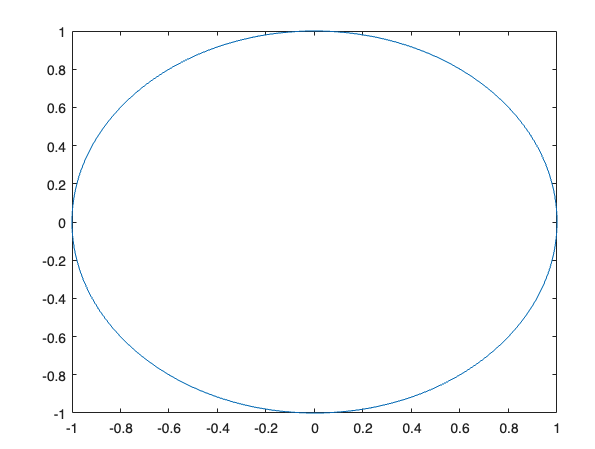
\includegraphics[scale = 0.6, center]{./Ortskurve_3_1.png}
					\caption{Ortskurve für unseres T-Glied}
					\label{fig3: Ortskurve}
				\end{figure}
\newpage
			\subsubsection{a.2}
				$$G(s) = \frac{K\cdot e^{-Ts}}{(1+T_1\cdot s)}$$
				\\
				$$G(j\omega) = \frac{K\cdot e^{-Tj\omega}}{(1+T_1\cdot j\omega)}$$
				\begin{figure}[h]
					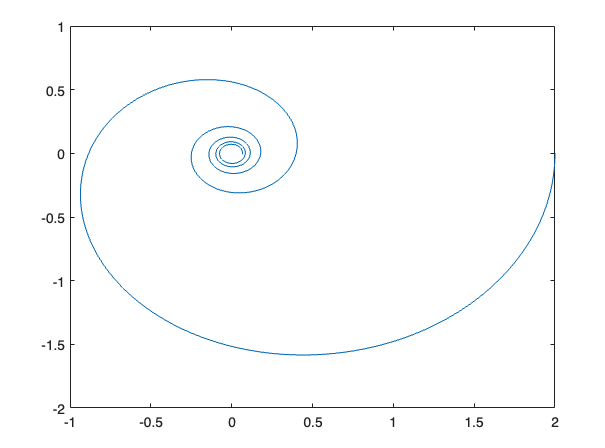
\includegraphics[scale = 0.7, center]{./Ortskurve_3_2.png}
					\caption{Ortskurve für unseres T-Glied}
					\label{fig3: Ortskurve}
				\end{figure}
\newpage
			\subsubsection{a.3}
				$$G(s) = \frac{K\cdot e^{-Ts}}{s(1+T_1\cdot s)}$$
				\\
				$$G(j\omega) = \frac{K\cdot e^{-Tj\omega}}{j\omega(1+T_1\cdot j\omega)}$$ 
				\begin{figure}[h]
					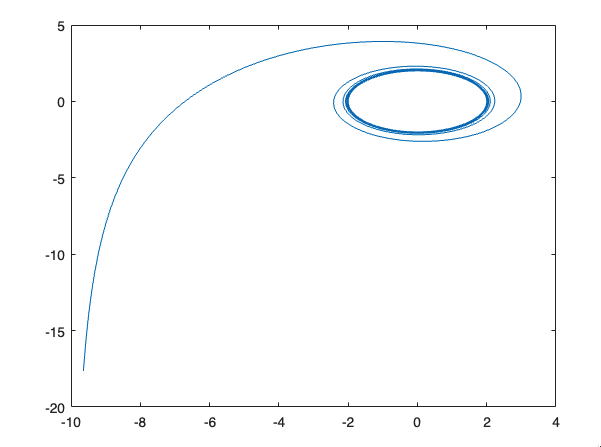
\includegraphics[scale = 0.7, center]{./Ortskurve_3_3.png}
					\caption{Ortskurve für unseres T-Glied}
					\label{fig3: Ortskurve}
				\end{figure}
\newpage
			\subsubsection{a.4}
				$$G(s) = \frac{K(T_vs+1)}{T_2s^2 + T_1s + 1}$$
				\\
				$$G(j\omega) = \frac{K(T_vj\omega + 1)}{T_2(j\omega)^2 + T_1j\omega + 1}$$
				\begin{figure}[h]
					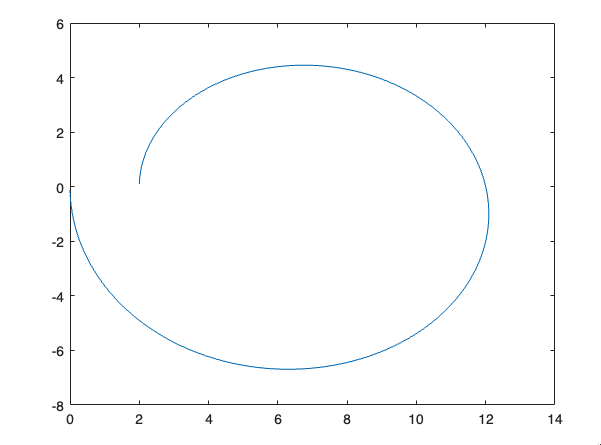
\includegraphics[scale = 0.7, center]{./Ortskurve_3_4.png}
					\caption{Ortskurve für unseres T-Glied}
					\label{fig3: Ortskurve}
				\end{figure}
\newpage
		\subsection{Grundverhalten der Regelglieder}		
			\subsubsection{b.1}
				Die erste Übertragungsfunktion besitzt das Grundverhalten eines T-Glied/Totzeitglied.
			\subsubsection{b.2}
				Die zweite Übertragungsfunktion besitzt das Grundverhalten eines $PT_1$-Glieds.
			\subsubsection{b.3}
				Die dritte Übertragungsfunktion besitzt das Grundverhalten eines $IT_1$-Glieds.
			\subsubsection{b.4}
				Die vierte Übertragungsfunktion besitzt das Grundverhalten eines $PT_2$-Glieds. 
				
	\section{Aufgabe 4: MATLAB Control System Toolbox}
		\subsection{Grund-Übertragungsverhalten}
			Die einzelnen Glieder verhalten sich wie folgt:
			\begin{itemize}
				\item $$G_R = K_R$$ ist eine \textbf{Konstante}.
				\item $$G_1 = \frac{F_0}{T_0^2 s^2 + 2DT_0 s +1}$$ zeigt das Verhalten eines \textbf{PT-2 Glieds}.
				\item $$G_2 = \frac{1}{K_L (1+T_s)}$$ verhält sich wie ein \textbf{PT-1 Glied}.
				\item $$G_3 = \frac{1}{s}$$ handelt nach einem \textbf{I-Glied}.
				\item $$G_{RADAR} = K_{RADAR}$$ ist wieder \textbf{konstant}.
			\end{itemize}
		\subsection{$G_O$ Übertragungsfunktion des offenen Regelkreises}
			Für die Übertragungsfunktion $G_O$ werden alle Teilglieder nacheinander multipliziert.
			$$G_O = G_{RADAR} \cdot G_R \cdot G_1 \cdot G_2 \cdot G_3$$
		
		\subsection{Ortskurve $G_O$}
			Um mit der erstellt Formel für $G_O$ die zugehörige Ortskurve zu erstellen, muss diese in MATLAB wie in folgendem Code angepasst werden.\\
			Der Befehle \lstinline{nyquist} in Zeile 18 plotet den Graphen.
			\begin{lstlisting}
				// Konstanten
				KRadar = 1;
				F0 = 1000;
				T0 = 1;
				D = 0.5;
				T1 = 1;
				KL = 1000;
				GR = 0.1;
				// Uebertragungsfunktion
				G1 = tf(F0 ,[T0^2 2*D*T0 1]);
				G2 = tf(1, [KL KL*T1]);
				G3 = tf(1, [1 0]);
				GRadar = tf(KRadar, 1);
				GO = series(series(series(series(GRadar,GR),G1),G2),G3);
				nyquist(G0);
			\end{lstlisting}
\newpage
			\begin{figure}[h]
				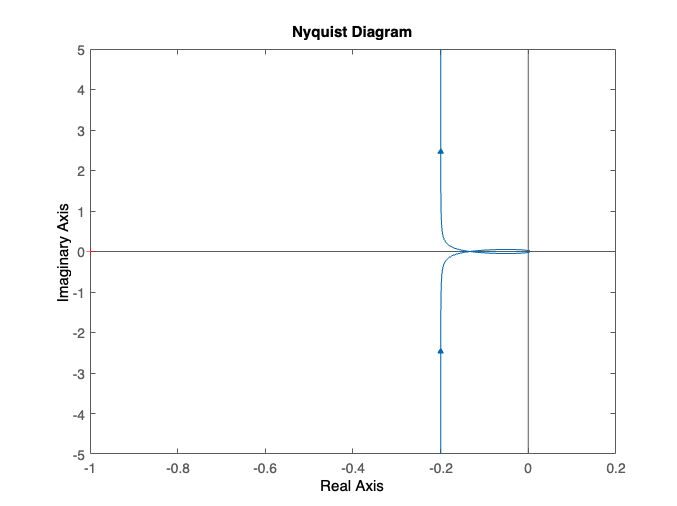
\includegraphics[scale=0.7, center]{./Ortskurve_4_c.png}
				\caption{Ortskurve für die Übertragungsfunktion $G_O$ des offenen Regelkreises.}
				\label{fig4: Ortskurve $G_O$}
			\end{figure}
\newpage
		\subsection{Übertragungsfunktionen}
			Die Ortskurven für die gegebenen Werte $K_{Ri}$ werden mit folgendem Code geplotet:
			\begin{lstlisting}
				//Konstanten
				KRadar = 1;
				F0 = 1000;
				T0 = 1;
				D = 0.5;
				T1 = 1;
				KL = 1000;
				GR = 0.1;

				//Teilaufgabe d
				KR1 = 0.05;
				KR2 = 0.1;
				KR3 = 0.2;
				KR4 = 0.4;
				KR5 = 0.8;

				GO1 = getGO(KR1, F0,T0,D,T1,KL,KRadar);
				GO2 = getGO(KR2, F0,T0,D,T1,KL,KRadar);
				GO3 = getGO(KR3, F0,T0,D,T1,KL,KRadar);
				GO4 = getGO(KR4, F0,T0,D,T1,KL,KRadar);
				GO5 = getGO(KR5, F0,T0,D,T1,KL,KRadar);

				figure;
				nyquist(GO1, 'b', GO2, 'g', GO, 'r', GO4, 'c', GO5, 'm');
				axis([-1, 0.4, -3, 3])
				grid;

				function GO = getGO(KR, F0, T0, D, T1, KL, KRadar)
				    G1 = tf(F0 ,[T0^2 2*D*T0 1]);
					G2 = tf(1, [KL KL*T1]);
				    G3 = tf(1, [1 0]);
				    GRadar = tf(KRadar, 1);
				    GO = series(series(series(series(GRadar, KR), G1), G2), G3);
				end
			\end{lstlisting}
\newpage
			\begin{figure}[h]
			    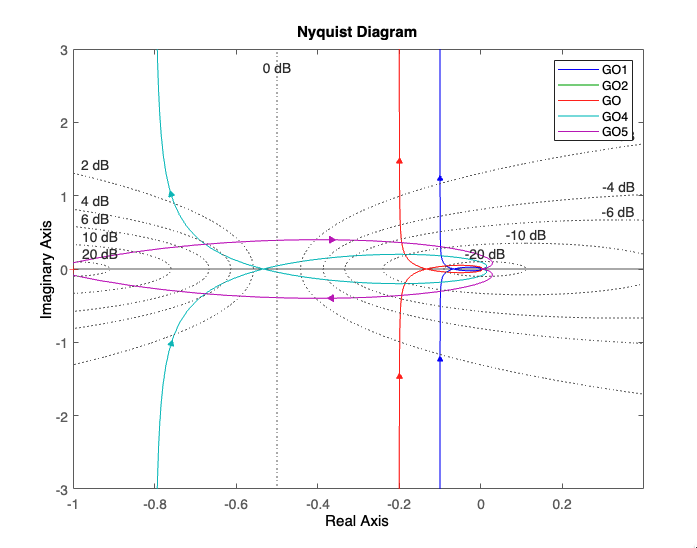
\includegraphics[scale=0.7, center]{./Ortskurven_4_d.png}
			    \caption{Ortskurven für die jeweiligen Werte für $K_R$.}
			    \label{fig:label}
			\end{figure}
\newpage
		\subsection{Bodediagramme}
			\begin{figure}[h]
			    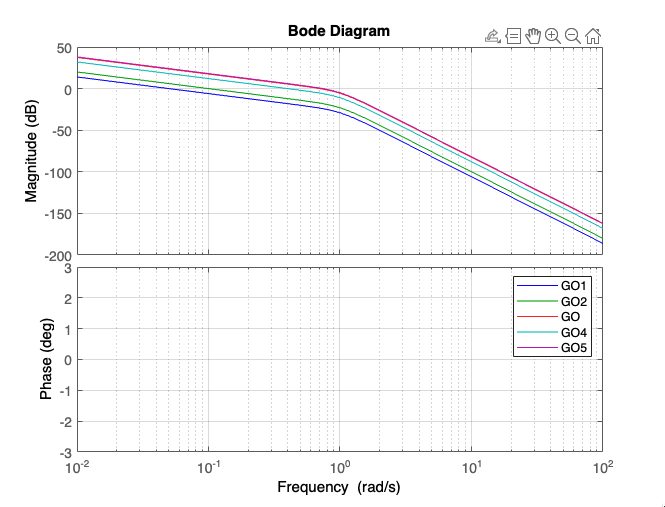
\includegraphics[scale=0.7, center]{./Bodediagramme_4_e.png}
			    \caption{Ortskurven für die jeweiligen Übertragungsfunktionen $G_{Oi}$.}
			    \label{fig:label}
			\end{figure}
\newpage
		\subsection{Bodediagramm des offenen Regelkreises mit \lstinline{margin}}
			\begin{figure}[h]
			    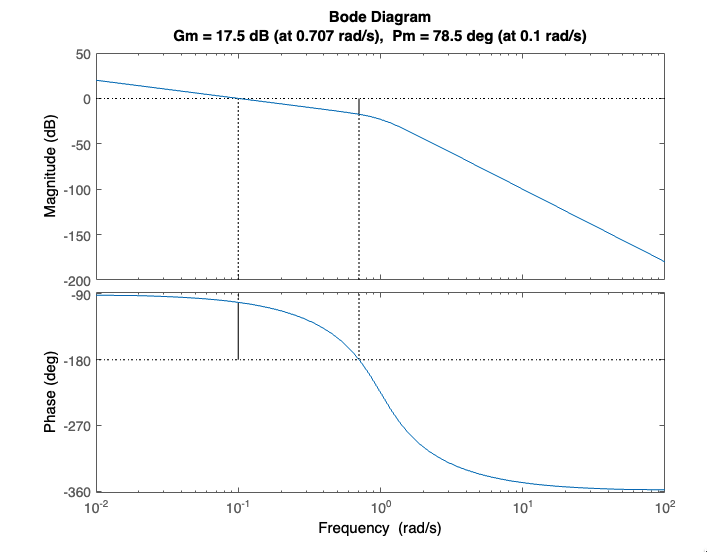
\includegraphics[scale=0.7, center]{./Bodediagramm_4_f.png}
			    \caption{Bodediagramm für die Übertragungsfunktion des offenen Regelkreises $G_O(s)$.}
			    \label{fig:label}
			\end{figure}
\newpage
			Mit dem gegebenen Code lässt sich ausprobieren, welchen Wert $K_R$ maximal annehmen darf.
			\begin{lstlisting}
				'Ergebnis: groesstes KR mit Stabilitaet ist ...'
				disp(KR_max);
				KR_range= 0.1:0.01:2;  //Vektor KR
				for i = 1:length(KR_range),
				    KR = KR_range(i);
				    GO = getGO(KR, F0,T0,D,T1,KL,KRadar);
				    // GM = Amplitudenreserve
				    // PM = Phasenreserve
				    // WGM = Winkel der Frequenz, bei der 0 dB geschnitten wird.
				    // WPM = Winkel der Frequenz, bei der 180 Grad geschnitten wird.
				    [GM, PM, WGM, WPM] = margin(GO);
				    if (GM<=1) || (PM<=0) || (WGM<=WPM)
				        KR_max = KR_range(i-1);
				        break;
				    end;
				end;
			\end{lstlisting}
			Die Schleife läuft über die Länge des Vektor KR, dessen Bereich von $0.1$ bis $2$ in $0.01$ großen Schritten, reicht. Dadurch wird jeder Wert nacheinander innerhalb der Schleife abgefragt und mit der Übertragsfunktion berechnet. Der Befehl \lstinline{margin} gibt damit die gesuchten Werte für Amplituden- und Phasenreserve wider; zusammen mit den dazugehörigen Winkelngrößen.\\
			Mit der \lstinline{if}-Abfrage bekommt man anschließend den gesuchten maximalen Wert zurück.
\newpage
			Der Komplette Code, der für diese Aufgabe verwendet wurde:
			\begin{lstlisting}
				KRadar = 1;
				F0 = 1000;
				T0 = 1;
				D = 0.5;
				T1 = 1;
				KL = 1000;
				GR = 0.1;

				G1 = tf(F0 ,[T0^2 2*D*T0 1]);
				G2 = tf(1, [KL KL*T1]);
				G3 = tf(1, [1 0]);
				GO = series(series(series(series(tf(KRadar, 1),GR),G1),G2),G3);

				// Bode-Diagramm plotten
				figure;
				bode(GO);
				// Gain- und Phase Margin berechnen
				margin(GO);
				[GM, PM, WGM, WPM] = margin(GO);
				disp(['Gain Margin (GM) in dB: ' num2str(GM)]);
				disp(['Phase Margin (PM) in degrees: ' num2str(PM)]);
				disp(['Gain Crossover Frequency (WGM) in rad/s: ' num2str(WGM)]);
				disp(['Phase Crossover Frequency (WPM) in rad/s: ' num2str(WPM)]);
		
				'Ergebnis: groesstes KR mit Stabilitaet ist ...'
				disp(KR_max);
				KR_range= 0.1:0.01:2;  //Vektor KR
				for i = 1:length(KR_range),
				    KR = KR_range(i);
				    GO = getGO(KR, F0,T0,D,T1,KL,KRadar);
				    [GM, PM, WGM, WPM] = margin(GO);
				    if (GM<=1) || (PM<=0) || (WGM<=WPM)
				        KR_max = KR_range(i-1);
				        break;
				    end;
				end;
				function GO = getGO(KR, F0, T0, D, T1, KL, KRadar)
				    G1 = tf(F0 ,[T0^2 2*D*T0 1]);
				    G2 = tf(1, [KL KL*T1]);
				    G3 = tf(1, [1 0]);
				    GRadar = tf(KRadar, 1);
				    GO = series(series(series(series(GRadar, KR), G1), G2), G3);
				end
			\end{lstlisting}
\newpage
			\subsection{Wurzelortskurve}
				\begin{lstlisting}
					KRadar = 1;
					F0 = 1000;
					T0 = 1;
					D = 0.5;
					T1 = 1;
					KL = 1000;
					GR = 0.1;
					k = 0.707; // entspricht 45 Grad
					G1 = tf(F0 ,[T0^2 2*D*T0 1]);
					G2 = tf(1, [KL KL*T1]);
					G3 = tf(1, [1 0]);
					GRadar = tf(KRadar, 1);
					GO = series(series(series(GRadar,GR),G1),G2);
					GCL1 = feedback(GO, G3);

					rlocus(GO);
					[K_opt, poles] = rlocfind(GO, k);
					disp(['Der optimale Verstaerkungsfaktor K betraegt: ' num2str(K_opt)])
				\end{lstlisting}
				\begin{figure}[h]
			    	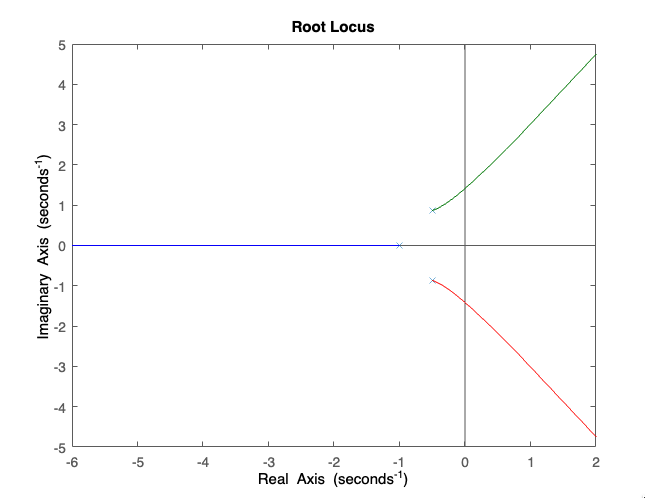
\includegraphics[scale=0.5, center]{./Aufg4_g_rootlocus.png}
				    \caption{Wurzelortskurven}
				    \label{fig:label}
				\end{figure}
\newpage
			\subsection{Übertragungsfunktionen der geschlossenen Regelkreise}
				\begin{lstlisting}
					// Konstanten
					KRadar = 1;
					F0 = 1000;
					T0 = 1;
					D = 0.5;
					T1 = 1;
					KL = 1000;
					GR = 0.1;

					// aus Teilaufgabe d
					KR1 = 0.05;
					KR2 = 0.1;
					KR3 = 0.2;
					KR4 = 0.4;
					KR5 = 0.8;

					GO1 = getGO(KR1, F0,T0,D,T1,KL,KRadar);
					GO2 = getGO(KR2, F0,T0,D,T1,KL,KRadar);
					GO3 = getGO(KR3, F0,T0,D,T1,KL,KRadar);
					GO4 = getGO(KR4, F0,T0,D,T1,KL,KRadar);
					GO5 = getGO(KR5, F0,T0,D,T1,KL,KRadar);

					// geschlossener Regelkreis
					GW1 = feedback(GO1, KRadar);
					GW2 = feedback(GO2, KRadar);
					GW3 = feedback(GO3, KRadar);
					GW4 = feedback(GO4, KRadar);
					GW5 = feedback(GO5, KRadar);

					function GO = getGO(KR, F0, T0, D, T1, KL, KRadar)
					    G1 = tf(F0 ,[T0^2 2*D*T0 1]);
					    G2 = tf(1, [KL KL*T1]);
					    G3 = tf(1, [1 0]);
					    GRadar = tf(KRadar, 1);
					    GO = series(series(series(series(GRadar, KR), G1), G2), G3);
					end
				\end{lstlisting}
				Nach diesem Code, mit Hilfe des Befehls \lstinline{feedback}, sehen die Übertragsfunktionen wie folgt aus:
				\subsubsection{$G_{O1} \rightarrow G_{W1}$}
					$$G_{W1} = \frac{50}{1000s^4 + 2000s^3 + 2000s^2 + 1000s + 50}$$
				\subsubsection{$G_{O2} \rightarrow G_{W2}$}
					$$G_{W2} = \frac{100}{1000s^4 + 2000s^3 + 2000s^2 + 1000s + 100}$$
				\subsubsection{$G_{O3} \rightarrow G_{W3}$}
					$$G_{W3} = \frac{200}{1000s^4 + 2000s^3 + 2000s^2 + 1000s + 200}$$
				\subsubsection{$G_{O4} \rightarrow G_{W4}$}
					$$G_{W4} = \frac{400}{1000s^4 + 2000s^3 + 2000s^2 + 1000s + 400}$$
				\subsubsection{$G_{O5} \rightarrow G_{W5}$}
					$$G_{W5} = \frac{800}{1000s^4 + 2000s^3 + 2000s^2 + 1000s + 800}$$
					
			\subsection{Impuls- und Sprungantworten}
 				\subsubsection{$G_{W1}$}
 					\begin{figure}[h]
 						\begin{subfigure}{0.5\textwidth}
 							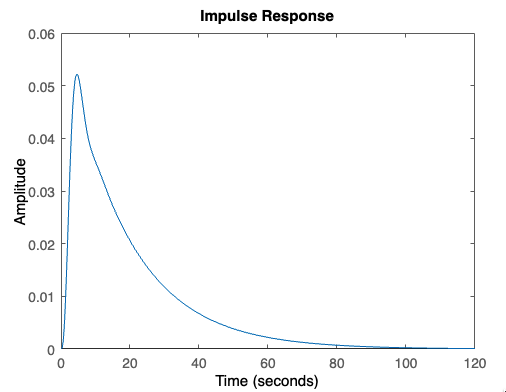
\includegraphics[width=1.2\linewidth]{./Impulsantwort_GW1.png}
						    \caption{Impulsantwort}
						    \label{fig:subimg1_1}
					    \end{subfigure}
					    \begin{subfigure}{0.5\textwidth}
					    		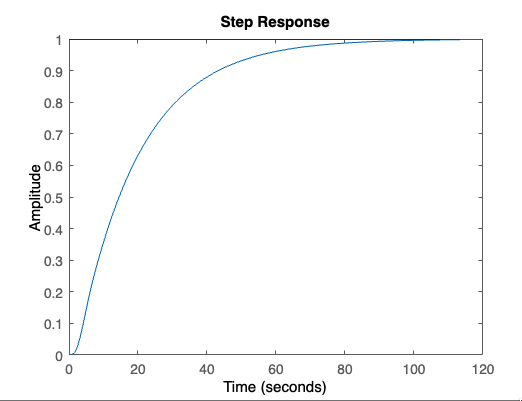
\includegraphics[width=1.2\linewidth]{./Sprungantwort_GW1.png}
					    		\caption{Sprungantwort}
					    		\label{fig:subimg1_2}
					    \end{subfigure}
 					\end{figure}
\newpage
 				\subsubsection{$G_{W2}$}
					\begin{figure}[ht]
 						\begin{subfigure}{0.5\textwidth}
 							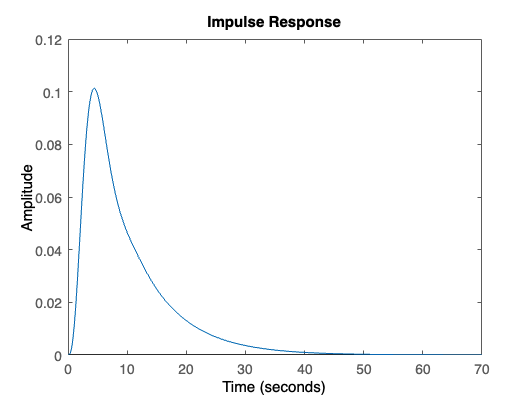
\includegraphics[width=1.2\linewidth]{./Impulsantwort_GW2.png}
						    \caption{Impulsantwort}
						    \label{fig:subimg2_1}
					    \end{subfigure}
					    \begin{subfigure}{0.5\textwidth}
					    		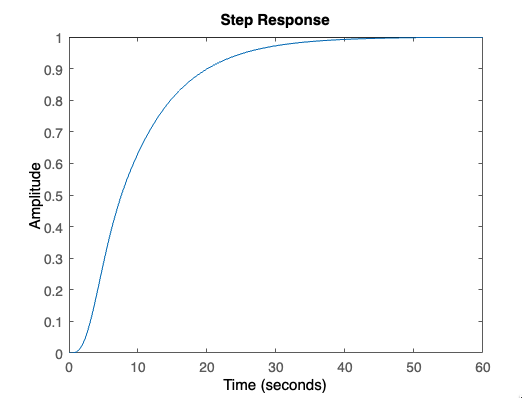
\includegraphics[width=1.2\linewidth]{./Sprungantwort_GW2.png}
					    		\caption{Sprungantwort}
					    		\label{fig:subimg2_2}
					    \end{subfigure}
 					\end{figure}
 				\subsubsection{$G_{W3}$}
 					\begin{figure}[h]
 						\begin{subfigure}{0.5\textwidth}
 							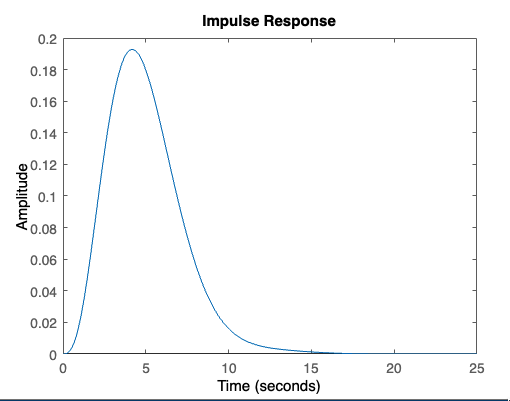
\includegraphics[width=1.2\linewidth, left]{./Impulsantwort_GW3.png}
						    \caption{Impulsantwort}
						    \label{fig:subimg3_1}
					    \end{subfigure}
					    \begin{subfigure}{0.5\textwidth}
					    		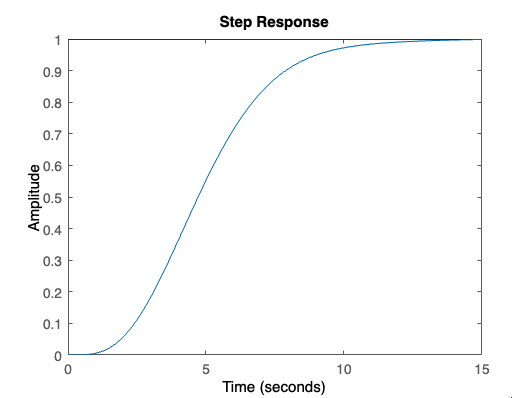
\includegraphics[width=1.2\linewidth]{./Sprungantwort_GW3.png}
					    		\caption{Sprungantwort}
					    		\label{fig:subimg3_2}
					    \end{subfigure}
 					\end{figure}
\newpage
 				\subsubsection{$G_{W4}$}
 					\begin{figure}[h]
 						\begin{subfigure}{0.5\textwidth}
 							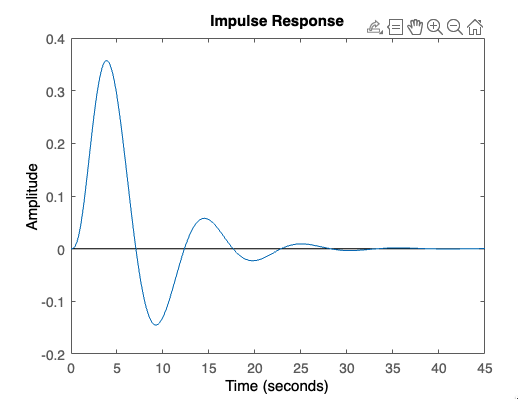
\includegraphics[width=1.2\linewidth]{./Impulsantwort_GW4.png}
						    \caption{Impulsantwort}
						    \label{fig:subimg4_1}
					    \end{subfigure}
					    \begin{subfigure}{0.5\textwidth}
					    		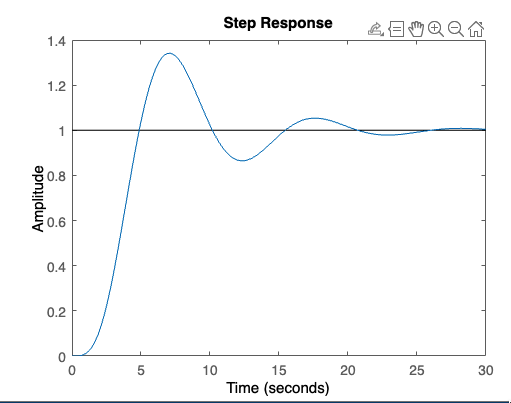
\includegraphics[width=1.2\linewidth]{./Sprungantwort_GW4.png}
					    		\caption{Sprungantwort}
					    		\label{fig:subimg4_2}
					    \end{subfigure}
 					\end{figure}
 				\subsubsection{$G_{W5}$}
 					\begin{figure}[h]
 						\begin{subfigure}{0.5\textwidth}
 							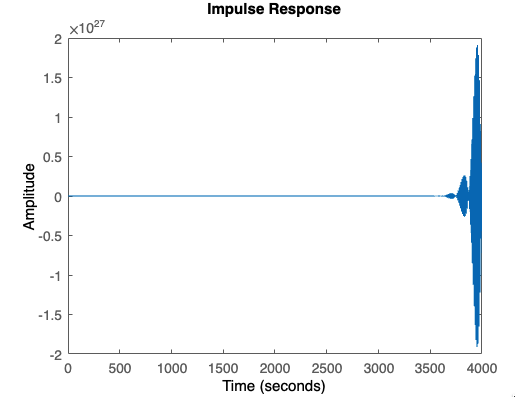
\includegraphics[width=1.2\linewidth]{./Impulsantwort_GW5.png}
						    \caption{Impulsantwort}
						    \label{fig:subimg5_1}
					    \end{subfigure}
					    \begin{subfigure}{0.5\textwidth}
					    		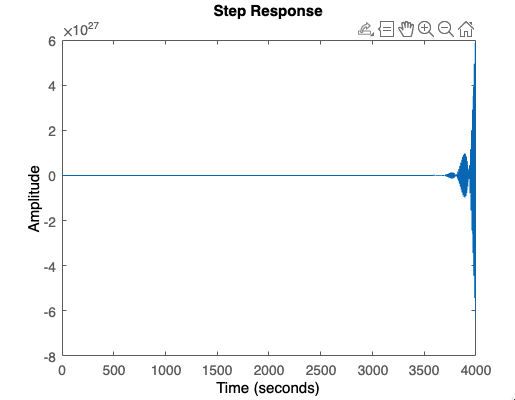
\includegraphics[width=1.2\linewidth]{./Sprungantwort_GW5.png}
					    		\caption{Sprungantwort}
					    		\label{fig:subimg5_2}
					    \end{subfigure}
 					\end{figure}
 				
\end{document}